\documentclass[12pt]{book}
\usepackage{graphicx}
\usepackage{mathtools}
\usepackage{xcolor}
\parindent 0pt
\parskip 6pt
\begin{document}
\title{
piHPSDR User's Manual
}
\author{
Christoph van W\"ullen, DL1YCF
}
%
\maketitle
\tableofcontents
\chapter{Introduction}
piHPSDR is a program that can operate with software defined radios (SDRs). As a graphical user interface,
it uses the GTK-3 toolkit, while the actual signal processing is done by Warren Pratt's WDSP library. Thus,
piHPSDR organizes the transfer of digitized radio frequency (RF) data between the radio hardware and the WDSP library, the
transfer of audio data (either from a microphone or to a headphone), as well as the processing of user
input (either by mouse/touch-screen, keyboard, or external "knobs and buttons"),
 and the graphical display of the RF data. piHPSDR is intended
to run on different variants of Unix. It runs on all sorts of Linux systems, including a Raspberry Pi (hence
the name piHPSDR), but equally well on Linux desktop or laptop computers, and on Apple Macintosh (Mac OSX)
computers which have a Unix variant under the hood. The present author is not aware of piHPSDR running
under the Windows operating system, although with environments such as MinGW, this should be possible.

Although piHPSDR can be operated entirely by using mouse and keyboard as input devices, many users prefer to
have physical push-buttons and/or knobs or dials. To this end, piHPSDR can control push-buttons and rotary
encoders connected to the GPIO (general purpose input/output)
lines of a Raspberry Pi. At least two generations of such controllers have
been put on the market by Apache labs, and I know of several projects where home-brewn controllers have
successfully been made. As an alternative, MIDI devices can be used for user interaction. For desktop/laptop
computers that do not have GPIO lines, MIDI offers an easy-to-use possibility of having push-bottons and
dials that control piHPSDR. Apart from homebrew projects in which a micro-controller such as an Arduino Micro
controls the actual buttons/knobs and acts as a MIDI device to the computer to which it is connected via USB,
there are low-cost so-called "DJ controllers" (DJ stands for disk jockey) from various brands which have
successfully been used with piHPSDR. A third possibility to control piHPSDR is via a serial interface
through CAT (computer aided transceiver) commands. The CAT model used by piHPSDR is based on the Kenwood
TS-2000 command set with lots of PowerSDR extensions.

Using a touch-screen instead of a mouse offers the possiblity to put the actual radio hardware together
with a Raspberry Pi running piHPSDR and an assortment of buttons/knobs into a single enclosure. This way,
one can build an SDR radio which can be operated like a conventional analog one.

The piHPSDR program has been written by John Melton G0ORX/N6LYT. It is free software that is licensed under
the GNU (free software foundation) general public license. Many other radio amateurs have contributed to
the code. A lot of extensions and improvements have been added by myself, therefore this document refers
to the version of piHPSDR that can be found on my github account \texttt{https://github.com/dl1ycf/pihpsdr}.

Because piHPSDR can be used on many different types of computers, and because operating systems change
rather quickly over time, I generally do not recommend to have a ,,binary release'' with files that you
can just copy to your computer and then it runs. Instead, my personal recommendation is to build piHPSDR
and WDSP from the sources, only this procedure guarantees compatibility of the final program with your
operating system. A manual of how to compile piHPSDR from the sources is available separately,
see \texttt{https://github.com/dl1ycf/pihpsdr-compile-from-sources}, so this will not be covered in 
the present manual. This manual starts with the first invocation of a freshly compiled piHPSDR.

\chapter{Starting piHPSDR for the first time}
Let us assume you have an SDR (say, an ANAN-7000 or a HermesLite-II) powered up and connected to an antenna,
and you have piHPSDR installed on a computer (say, a Raspberry Pi or an Apple Macintosh), the first thing to
do is to establish a proper connection between the computer and the radio. Although advocated at many places,
I do highly recommend against a WiFi connection. WiFi routers often use ,,optimizations'' where they hold
back data packets for a given client for a while, to be able to send a collection of them in a burst. While
this certainly optimizes the through-put because it minimizes clear-channel arbritration events, such jitters
are desastrous in SDR operation. The safest way of connecting the radio and the computer is to have a
managed switch with a built-in DHCP server, and to connect both the computer and the radio with a suitable
cable to the switch. If the computer has both a RJ45 jack for an ethernet cable, and a WiFi interface, my
personal recommendation is to use WiFi to connect to the internet, and use a single ,,direct cable'' plugged
into the RJ45 jacks of the computer and of the radio. This is a little bit tricky since both the computer
and the radio have to be set to a fixed IP address (e.g. computer: 192.168.1.50, radio: 192.168.1.51) with
the same netmask. However, once this has been done, this is the safest connection with no perturbations from
elsewhere.

\newpage
If the piHPSDR program is started for the first time, it opens a window that looks like this

\begin{center}
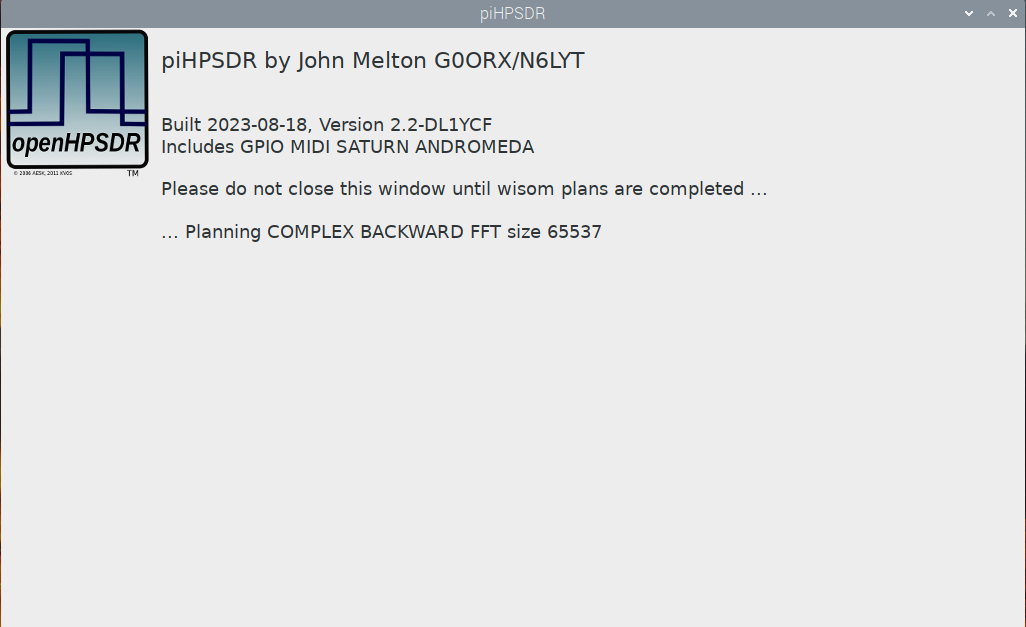
\includegraphics[width=12cm]{Planning.png}
\end{center}

besides stating a version number and when piHPSDR was built, a list of optional features (to be activated
at compile time) is stated, in this case, GPIO, MIDI, SATURN, and ANDROMEDA. These options indicate
that the program has GPIO support (this is only possible on Raspberry Pi or similar single board computers),
that is has support for MIDI devices, that it can run natively on the compute module of the latest
G2 (generation two) SDRs from Apache labs, and that is has support for Laurence Barker's ANDROMEDA controller.
What is important here that you have to wait. This only applies to the very first time you start piHPSDR.
On CPUs with a rather simple instruction set (like the ARM processor in the Raspberry Pi, or the Apple
Silicon processor in recent Macintosh computers), this "planning" step is quite fast, on CPUs with very
complex instruction sets like the Intel x86 processors, this step can last up to 15 minutes. When the
"wisdom plans" are completed, piHPSDR tries to detect a radio on the network. If everything went well with
the network connection, you then see a screen with a ,,discovery menu''

\begin{center}
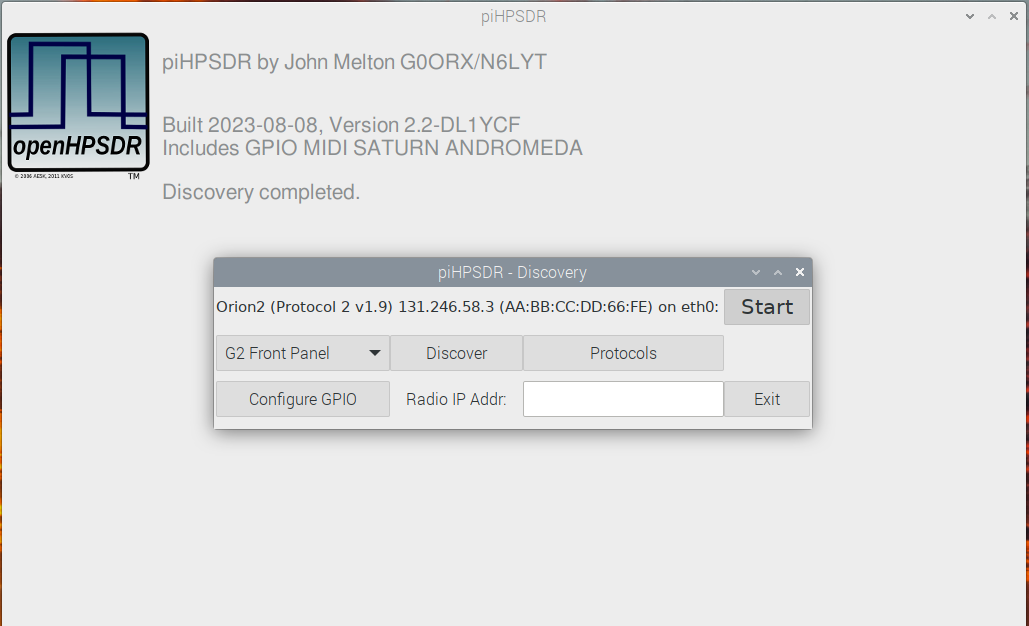
\includegraphics[width=12cm]{Start.png}
\end{center}

At this point, you can start the radio by clicking the "Start" button, but let us first explain the
purpose of the other buttons! Easiest to explain is the "Exit" button, this will simply terminate
the program. Most likely, you may want to go into the "Protocols" menu. By default, piHPSDR tries to
,,discover'' a radio using all protocols known to piHPSDR. However, if you know that your radio, for
example, uses Protocol 2, then trying to discover a Protocol-1 radio is just a waste of time. So if you
know which types of radio you want to connect to, check these protocols. The available protocols are 
\end{document}
